\documentclass[12pt]{article}

\usepackage[]{graphicx}
\usepackage[]{color}
\usepackage{alltt}
\usepackage{amsmath}
\usepackage{amssymb}
\DeclareMathOperator{\diag}{diag}
\DeclareMathOperator{\pen}{pen}

\newcommand{\mytitle}{Survey on Regularization Methods in Continual Learning}
\newcommand{\myname}{Jörg Schantz}
\newcommand{\mysupervisor}{Dr. Julian Rodemann}

\usepackage[a4paper, width = 160mm, top = 35mm, bottom = 30mm, 
bindingoffset = 0mm]{geometry}
\usepackage[utf8]{inputenc}
\usepackage{ragged2e}
\usepackage{xcolor}
\usepackage[numbers, sort&compress]{natbib}
\usepackage{fancyhdr}
\newcommand{\changefont}{%
	\fontsize{8}{11}\selectfont
}
\usepackage{hyperref}
\hypersetup{
	colorlinks = true,
	linkcolor = black,
	urlcolor = black,
	citecolor = black}
\pagestyle{fancy}
\fancyhead{}
\fancyhead[R]{\changefont{\mytitle}}
\fancyfoot{}
\fancyfoot[R]{\thepage}
\setlength{\headheight}{14.5pt}
\setlength{\parindent}{0pt}
\interfootnotelinepenalty = 10000
\usepackage{setspace}
\onehalfspacing

% ------------------------------------------------------------------------------
% MAIN -------------------------------------------------------------------------
% ------------------------------------------------------------------------------
\IfFileExists{upquote.sty}{\usepackage{upquote}}{}
\begin{document}
	
	% FRONT PAGE -------------------------------------------------------------------
	
	\begin{titlepage}
		\begin{center}
			
			\LARGE
			Bachelor's Thesis
			
			\vspace{0.5cm}
			
			\rule{\textwidth}{1.5pt}
			\LARGE
			\textbf{\mytitle}
			\rule{\textwidth}{1.5pt}
			
			\vspace{0.5cm}
			
			\large
			Department of Statistics \\
			Ludwig-Maximilians-Universität München 
			
			\vfill
			
			\Large
			\textbf{\myname}
			
			\vfill
			
			\large
			Munich, March 20\textsuperscript{th}, 2025
			
			\vfill
			
			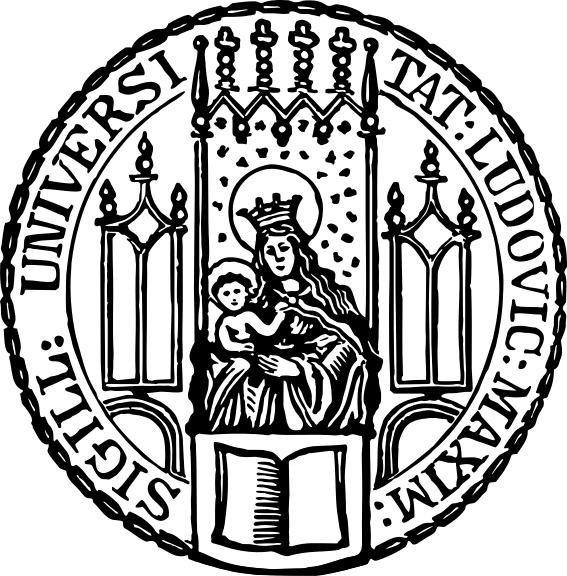
\includegraphics[width = 0.4\textwidth]{img/sigillum.png}
			
			\vfill
			
			\normalsize
			Submitted in partial fulfillment of the requirements for the degree of B. Sc.
			\\
			
			Supervised by \mysupervisor
			
		\end{center}
	\end{titlepage}
	
	% CONTENTS ---------------------------------------------------------------------
	
	\pagenumbering{Roman}
	\newpage
	
	\begin{abstract}
		
		Lorem ipsum dolor sit amet, consectetur adipiscing elit, sed do eiusmod tempor 
		incididunt ut labore et dolore magna aliqua. Ut enim ad minim veniam, quis 
		nostrud exercitation ullamco laboris nisi ut aliquip ex ea commodo consequat. 
		Duis aute irure dolor in reprehenderit in voluptate velit esse cillum dolore eu 
		fugiat nulla pariatur. Excepteur sint occaecat cupidatat non proident, sunt in 
		culpa qui officia deserunt mollit anim id est laborum. \cite{SB}
		
	\end{abstract}
	
	\newpage
	\tableofcontents
	
	%%%% if you would want to include material overview
	%%%% use one of the following in addition
	% \newpage
	% \listoffigures
	% \newpage
	% \listoftables
	\newpage
	
	% CHAPTERS ---------------------------------------------------------------------
	
	\pagenumbering{arabic}
	
	\section{Introduction}
	\label{intro}
	%%%%%%%%%%%%%%%%%%% Introduction %%%%%%%%%%%%%%%%%%%
The internet has opened many doors for humanity one of those being the apparent access to infinite information. Everyday people around the world generate over 400 million terabyte of new data \cite{matt2024}. This well of information has recently been adopted to train prominent artificial intelligence agents, like GPT-3 \cite{kashyap-2023}. Training these models even once is very expensive \cite{buchholz-2024} which makes it hard for developers to keep up with the seemingly unending flow of new data. Aside from this financial factor, the physical limitations of storage and computation time for all of these data files pose another problem for AI developers and demonstrates the need for selective model editing without retraining. On a smaller scale, AI often needs to adapt to more specialized use cases \cite{verwimp2024continuallearningapplicationsroad}. Pre-trained AI models, for example in smart watches, need to be able to adapt to their owner's habits in order to be fully functional.
Continual learning (CL), often referred to as lifelong learning or incremental learning, aims to solve ease these limitations for AI by dividing all available and future data into distinct sets, which are then processed sequentially \cite{verwimp2024continuallearningapplicationsroad}.

Training on distinct data sets, puts developers in front of a new problem: how can they make sure AI does not forget previously learned information? 

AI is built on artificial neural networks (ANN), a machine learning program, that makes decisions by mimicing a human brain \cite{ibm2025}. Although they are inspired by humans they currently lack the ability to look inward and reflect on themselves. Ergo, people need to find ways to determine what is important information for AI in order to enable efficient ways of "remembering". Understanding how ANNs make decisions is also important to build trust and confidence in AI \cite{Sudmann2020}. 

Their use cases go far beyond suggesting a new song for your playlist or correcting typos in a rushed text message. We have started to implement AI to drive cars or help with medical examinations. These tasks often come with variations, like driving in different weather conditions or recognizing more than one kind of tumor. It would be desirable to have a single AI that can learn these task when required and maybe even use previously learned information to help with the new training process. Like children first learn the alphabet and then use this knowledge to read and write texts, AI should leverage prior tasks to solve new ones.

Throughout this thesis I want to explore the possibilities and limitations of regularization as a CL method with some selected examples, as well as how advances in this field can contribute to a better understanding of ANNs. There have been thorough surveys on CL as a whole \cite{LW, verwimp2024continuallearningapplicationsroad, bidaki2025}, which provide a more complete overview of this field. This thesis separates itself from them by diving deeper into individual methodologies in order to demonstrate how regularization in CL has helped to extract importance measures in ANNs and which tasks can even be learned in such a setting.
	\section{Neural Networks}
	\label{nn}
	Although continual learning is general modeling concept, applicable in statistical inference as well as pattern driven prediction algorithms, it is mostly used a in machine learning context. More specifically in artificial neural networks (ANN). They are algorithms based on the functionality of a human brain and often designed for scenarios where data is seen in real-time e.g. stock market predictions or power control systems.\\
The simplest form of an ANN is a single linear classifier, called one-neuron perceptron, that devides a vector $x$ into two classes using a so-called activation function $h(\cdot)$ \cite{Du_2019}. The neuron's input is given by
\begin{equation}
	\sum_{i = 1}^{n}{w_i x_i}+c = w^\top x+c
\end{equation}
where $n$ is the number of observations, $w$ a weight vector assigned to $x$ and $c$ the decision threshold. The two class regions are separated by the hyperplane \cite{Du_2019}
\begin{equation}
	w^\top x + c = 0
\end{equation}.
Using multiple neurons with the same activation function creates a one-layer perceptron and enables classification for more than two classes with the input
\begin{equation}
	\sum_{k = 1}^{m}\sum_{i=1}^{n}w_{k,i}x_i + c = (w_1^\top x + c, ..., w_m^\top x + c)^\top = W^\top x + c
\end{equation} 
where $W$ is the $n\times m$ weight matrix and $m$ the number of classes. Given $h$ the logistic function a one-layer perceptron is equal to a multinomial logit model \cite{Fahrmeir_2022}. Composing $l$ layers of neurons, Feed Forward NN (FFNN), allows for a more and more abstract representation of the data and finer class boundaries. The unknown weight matrices $W_1, ..., W_l$ and the decision threshold $c$ are the solution to the minimization problem
\begin{equation}
	\hat{\theta} = \arg\min{\sum_{i=1}^{n} L(f(x_i, \theta), y_i)}
\end{equation}
where $\theta$ are the unknown parameters, and $L(\cdot)$ a loss function which measures the difference between the predicted values $f(x_i, \theta)$ and true values $y_i$.\\
%-------------
% ADD PICTURE
%-------------
	\section{Framework}
	\label{framework}
	
We are interested in optimizing the parameters theta of a single neural network to perform well across
multiple tasks $D_1, ...,D_T$ , specifically finding a MAP estimate $\theta^*=\arg\max_\theta p(\theta|D_1,...,D_T)$.
However, the datasets arrive sequentially and we can only train on one of them at a time.
In the following, we first discuss how Bayesian online learning solves this problem and introduce an
approximate procedure for neural networks. We then review recent Kronecker factored approxima-
tions to the curvature of neural networks and how to use them to obtain a better fit to the posterior.
Finally, we introduce a hyperparameter that acts as a regularizer on the approximation to the posterior.\\
Bayesian online learning [31 ], or Assumed Density Filtering [25 ], is a framework for updating an
approximate posterior when data arrive sequentially. Using Bayes’ rule we would like to simply
incorporate the most recent dataset D into the posterior as:
\begin{equation}
	E = mc^2
\end{equation}
where we use the posterior D from the previously observed tasks as the prior over the
parameters for the most recent task. As the posterior given the previous datasets is typically intractable,
Bayesian online learning formulates a parametric approximate posterior q with parameters pi, which
it iteratively updates in two steps:
Update step In the update step, the approximate posterior q with parameters pi from the previous
task is used as a prior to find the new posterior given the most recent data:
\begin{equation}
	E = mc^2
\end{equation}
Projection step The projection step finds the distribution within the parametric family of the
approximation that most closely resembles this posterior, i.e. sets pi such that:
\begin{equation}
	E = mc^2
\end{equation}
Opper and Winther [31] suggest minimizing the KL-divergence between the approximate and the
true posterior, however this is mostly appropriate for models where the update-step posterior and a
solution to the KL-divergence are available in closed form. In the following, we therefore propose
using a Laplace approximation to make Bayesian online learning tractable for neural networks:
	\subsection{Scenarios}
	\label{scenarios}
	%%%%%%%%%%%%%%%%%%% Scenarios %%%%%%%%%%%%%%%%%%%
In regards to the distribution $\mathbb{P}$ of $Y^{(t)} = \{Y_1, ..., Y_t\}$ over which the model is evaluated after seeing the $t$-th samples, \cite{bidaki2025} and \cite{LW} differentiate between eight CL scenarios:\\
\textit{Task-incremental learning} (TIL), \textit{Class-incremental learning} (CIL), \textit{Task-Free continual learning} (TFCL) and \textit{Online contiunal learning} (OCL) algorithms all aim to learn a distinct set of tasks, while providing a task identity, if not stated otherwise \cite{bidaki2025, LW}.
\begin{equation}
	\emptyset = Y_t \cap Y_{t+1} \Rightarrow \mathbb{P}(Y^{(t+1)}) = \prod_{i = 1}^{t+1}\mathbb{P}(Y_i)
\end{equation}
TIL allows task individual output layers or the training of separate models for each task. The challenge then is less about forgetting (\autoref{cf}) but finding a healthy balance between predicting accuracy and model complexity \cite{vandeVen2022}.\\
CIL restricts this approach by only training one model, which is introduced stepwise to different classification tasks. CIL only provides task identity during training \cite{vandeVen2022}. For example with samples $t$ an agent learns to classify hats or gloves and with sample $t+1$ shirts or pants. When testing, it is then also required to classify hats or shirts.\\
TFCL does not provide any task identity to the model and only focuses on labels \cite{aljundi2019tfcl}.\\
OCL limits its sample sizes to one and focuses on real-time training \cite{bidaki2025, LW}.\\
\textit{Domain-incremental learning} (DIL) algorithms seek to learn multiple tasks that share the same label space [\citenum{bidaki2025}]. For example first learning to drive during sunny weather and later on while it is rainy.
\begin{equation}
	Y_t=Y_{t+1} \nRightarrow \mathbb{P}(Y_t) = \mathbb{P}(Y_{t+1})
\end{equation}
One could view this as a version of task-incremental learning, where task identity is secondary as all tasks have the same data labels. Thus design based strategies to inhibit catastrophic forgetting are not possible \cite{vandeVen2022}.\\
\textit{Instance-incremental learning} (IIL) algorithms learn one common task for all training samples \cite{bidaki2025, LW}.
\begin{equation}
	Y_t=Y_{t+1}, \mathbb{P}(Y_t) = \mathbb{P}(Y_{t+1}) \Rightarrow \mathbb{P}(Y^{(t+1)})=\mathbb{P}(Y_1)
\end{equation}
This is a special case of DIL where a model learns the distribution of one "domain" while only ever accessing snippets of the total available data. For example each sample contains new real-world photographs of cats to classify. Assuming OCL only learns one task, OCL is a special case of IIL where every data point is seen in sequence.\\
\textit{Blurred Boundary continual learning} (BBCL), in contrast to all others so far, allows partially overlapping label spaces \cite{bidaki2025,LW}.\\
\textit{Continual Pre-training} (CPT) aims to improve knowledge transfer with sequentially arriving pre-training data \cite{bidaki2025, LW}.
	\subsection{Stability-Plasticity Trade-off}
	\label{cf}
	%%%%%%%%%%%%%%%%%%% Stability-Plasticity Trade-off %%%%%%%%%%%%%%%%%%%
The challenge of continual learning is to strike a balance between stability and plasticity. Models should retain knowledge of past tasks, stability, while being flexible enough to incorporate information from new data, plasticity. The sequential training nature of CL changes the weights acquired form learning task A to accommodate for a new task B. This abrupt loss of information is called catastrophic forgetting \cite{FRENCH1999128, Mcclelland1995, MCCLOSKEY1989109, Ratcliff1990ConnectionistMO}. A naive approach to solving this dilemma would be storing and replaying data to the network with each training step. This is impractical because the amount of data needed to be stored is proportional to the number of tasks learned.\\
\citeauthor{evron2022} define forgetting as
\begin{equation}
	F(k) = 1/k \sum_{t=1}^{k}\lVert X_t w_k - y_t \rVert^2
\end{equation}.
They have analyzed catastrophic forgetting in linear regression under the assumptions that values of $X$ are bounded by 1, tasks are jointly realizable with a bounded (by 1) norm and there are more parameters than observations in each sample. Realizability assumes the existence of true model weights s.t. $y =Xw$ \cite{Shalev-Shwartz}. This enables them to focus only on minimizing the distance between new and old model weights. In their work they find an upper bound for forgetting
\begin{equation}
	\sup F(k) = \sup 1/k \sum_{k}^{t=1}\lVert(I-Q_t)Q_k ... Q_1\rVert^2
\end{equation}
where $Q_i$ are the projections onto the solution spaces of $w_i$ i.e. $Q_i := I - X_i^\top(X_i X_i^\top)^{-1} X_i$.\\
So far many methods of minimizing catastrophic forgetting have been developed. Their core ideas can be summarized to \textit{Replay} methods \cite{chaudhry2019,rebuffi2017icarlincrementalclassifierrepresentation, aljundi2019gradientbasedsampleselection}, \textit{Optimization} methods \cite{lopezpaz2022gradientepisodicmemorycontinual, javed2019metalearningrepresentationscontinuallearning, mirzadeh2020understandingroletrainingregimes}, \textit{Architecual} methods \cite{mallya2018piggybackadaptingsinglenetwork, ebrahimi2020adversarialcontinuallearning, fernando2017pathnetevolutionchannelsgradient} and \textit{Regularization} methods, which will be discussed in \autoref{}. 

	\section{Metrics}
	\label{metrics}
	%%%%%%%%%%%%%%%%%%% Metrics %%%%%%%%%%%%%%%%%%%
Intro.\\
In the following each sample $D_t = (X^{(t)}, y^{(t)})$ is divided into a training split $D_t^{(train)} = (X^{(t)}_{(train)}, y^{(t)}_{(train)})$ and a testing split $D_t^{(test)} = (X^{(t)}_{(test)}, y^{(t)}_{(test)})$. The chosen splitting method is arbitrary. The training process for each sample will be conducted with $D_t^{(train)}$ and evaluation with $D_t^{(test)}$.\\
\cite{LW} mention different measures for model performance, stability and plasticity. I will focus on the dynamic forms given by \cite{díazrodríguez2018dontforgetforgettingnew}, because they are adapted for in training use i.e. they represent a model's current state after the $t$-th training step.\\
\textit{Accuracy} $\mathbf{A}$ represents a models performance i.e. how well the predictions $\hat{y}^{(t)}_{(test)}$ align with the true values of $y^{(t)}_{(test)}$ for a metric $\mu$ . When $A_{i,k}$ is the accuracy measured on the $k$-th test split after the $i$-th training step, then
\begin{equation}
	\mathbf{A} = \frac{2}{t(t-1)}\sum_{i \geq k }^{t} A_{i,k}
\end{equation}
is the average accuracy after the $t$-th training step over all test splits $D_k^{(test)}, k <= t$ \cite{díazrodríguez2018dontforgetforgettingnew}.\\
\textit{Backward Transfer} $\mathbf{BWT}$ evaluates a models stability \cite{LW}. The metric quantifies the influence of learning sample $D_{t+1}^{(train)}$ has on the performance over test sample $D_t^{(test)}$ \cite{lopezpaz2022gradientepisodicmemorycontinual}. Given, the above mentioned, individual \textit{Accuracy} scores $A_{i,k}$
\begin{equation}
	\mathbf{BWT} = \frac{2}{t(t-1)} \sum_{i=2}^{t}\sum_{k=1}^{i-1}(A_{i,k}-A_{k,k})
\end{equation}
is the average backward transfer after the $t$-th training step \cite{díazrodríguez2018dontforgetforgettingnew}. Note that $\mathbf{BWT}$ can be negative. This property captures (catastrophic) forgetting \cite{LW}.\\
\textit{Forward Transfer} $\mathbf{FWT}$ is a metric for model plasticity \cite{LW}. Complementary to BWT, \textit{Forward Transfer} measures how previous training steps influence the current one. Again the individual \textit{Accuracy} scores are the basis for this evaluation metric. The average influence of old training steps on the model performance after the $t$-th step:
\begin{equation}
	\mathbf{FWT} = \frac{2}{t(t-1)}\sum_{i < k }^{t} A_{i,k}
\end{equation}
\cite{díazrodríguez2018dontforgetforgettingnew}.\\
Another metric that directly measures the relationship between stability and plasticity is presented in \cite{mirzadeh2020understandingroletrainingregimes}. The authors use the maximum eigenvalue of the loss' Hessian $\lambda^{max}$ to describe the width of their approximation of the loss' minimum. They hypothesize that the \textit{wideness} of this minimum correlates with the forgetting rate of the respective model.\\
Given $W^{(t)*}$ and $W^{(t+1)*}$ the optimal parameters after learning the $t$-th and $t+1$-th task and $L_t(\cdot)$ and $L_{t+1}(\cdot)$ the corresponding loss functions. \citeauthor{mirzadeh2020understandingroletrainingregimes} formulate the upper bound
\begin{equation}\label{2TA}
	F_t = L_t(W^{(t+1)*}) - L_t(W^{(t)*}) \approx \frac{1}{2}{\Delta W}^\top \nabla^2 L_t(W^{(t)*}) \Delta W \leq \frac{1}{2}\lambda_t^{max}\lVert \Delta W \rVert^2
\end{equation}
for the forgetting $F_t$ of the $t$-th task. They approximate $L_t(W^{(t+1)*})$ around $W^{(t)*}$ with a second order Taylor approximation, where $\nabla^2$ is the Hessian for $L_t$ and $\Delta W$ the difference between $W^{(t+1)*}$ and $W^{(t)*}$. They argue that the loss can be approximated this way, because of its almost convex path around the minimum, for models that have more observations per sample than parameters.\\
Further, ${\Delta W}$ is dependent on the training process of the $t+1$-th task, which depends on the random sample it is trained on, so one can view the differences in parameters as a random vector, that follows some distribution parameterized by the eigenvalues of $\nabla^2 L_t(W^{(t)*})$ \cite{mirzadeh2020understandingroletrainingregimes}.\\

Controlling the distance of the weights seems to be the key to mitigating forgetting...
	\section{Regularization}
	\label{reg0}
	%%%%%%%%%%%%%%%%%%% Regularization %%%%%%%%%%%%%%%%%%%
As mentioned in \autoref{cf}, one way to address the stability-plasticity problem is the use of regularization. This approach adds a penalty term to the loss function of a model. Usually this penalty term depends on the model parameters. Later we will also see some methods that directly penalize the output of a model. I will begin by categorizing the regularization methods that I have found through out my research and present some selected examples. After this overview of current possibilities in regularization techniques and present attempts at unifying and generalizing them.\\
In \cite{evron2022,li2024fixeddesignanalysisregularizationbased} the authors introduce a rudimentary approach to regularization in CL, \textit{ordinary conitunal learning}. It is used as a worst case comparison for their contribution to this field and is the basis for the upper bound on forgetting in \autoref{cf}.\\
Despite its limitations, I believe that it is a beneficial to start this section with ordinary CL. It reduces the complexity of neural networks to two linear regression problems, which makes for a softer entry into the field.\\
Assuming a CL problem with $T=2$ linear regression models $y^{(t)} = X^{(t)}w^* + \epsilon_t, \epsilon_t \sim N(0, \sigma^2), t \in \{1,2\}$, the task corresponding samples $D_t = (X^{(t)}, y^{(t)}) \in (\mathbb{R}^{n_t \times d}, \mathbb{R}^{n_t})$ and the commutable covariance matrices $\Sigma_t$. Then ordinary continual learning algorithm performs an ordinary least square (OLS) minimization over the first sample set $D_1$ to estimate the parameters $\hat{w}^{(1)} = (X^{(1)\top}X^{(1)})^{-1}X^{(1)\top} y^{(1)}$. In the second training sequence, ordinary CL fits $w^{(2)}$ to the residuals of task one with respect to $X^{(2)}$. The new parameters $\hat{w}^{(2)}$ are then:
\begin{equation}
	\hat{w}^{(2)} = \hat{w}^{(1)} + (X^{(2)\top}X^{(2)})^{-1}X^{(2)\top} (y^{(2)} - X^{(2)}\hat{w}^{(1)})
\end{equation}.
In their analysis of ordinary continual learning, \cite{li2024fixeddesignanalysisregularizationbased} show that it suffers from catastrophic forgetting when dealing with "dissimilar" tasks i.e. similarity is measured via the following bound:
\begin{equation}
	d_F \leq tr(\Sigma_1\Sigma_2^{-1})
\end{equation}
where $d_F$ is the expected forgetting rate between the two tasks.\\
Due to the heavy assumptions made, especially that both minimization problems have the common solution $w^*$, ordinary CL is only applicable in DIL and IIL. This highlights the need for methodologies that control weight deviation when trying to combat forgetting in a less restrictive setting.


	\subsection{Regularization via Parameters}
	\label{reg01}
	\subsubsection{Quadratic Penalties}
	\label{reg011}
	%%%%%%%%%%%%%%%%%%% Regularization via Parameters %%%%%%%%%%%%%%%%%%%
%%%%%%%%%%%%%%%%%%% L2 Norm %%%%%%%%%%%%%%%%%%%
%% L2 Continual Ridge Regression %% 
Expanding on the naive \textit{ordinary continual learning} approach, \citeauthor{li2024fixeddesignanalysisregularizationbased} suggest an adaptation of the Ridge penalty \cite{Fahrmeir_2022} for continual learning, dubbed \textit{continual ridge regression} (CRR) \cite{li2024fixeddesignanalysisregularizationbased, zhao2024statisticaltheoryregularizationbasedcontinual}. Again the $\hat{w}^{(t)}$ follow a Gaussian distribution $N(w^*, \sigma^2(X^{(t)\top} X^{(t)})^{-1})$ and the estimation of $w^{(1)}$ stays the same as in ordinary CL, too. For estimating $w^{(2)}$, they introduce now a ridge-like penalty term
\begin{equation}
	\pen(w) = \lambda\lVert w - \hat{w}^{(1)}\rVert_2^2
\end{equation}
which centers the new weights around the previously estimated $\hat{w}^{(1)}$ instead of 0. Instead of using penalized least squares, the authors decide to perform a penalized mean squared error regression. %% change to MSE in Reg0 chapter
\begin{equation}
	\begin{split}
		\hat{w}^{(2)} &= \arg\min_{w} \frac{1}{n}\lVert y^{(2)} - X^{(2)}w\rVert_2^2 + \pen(w) \\
		&= (X^{(2)\top} X^{(2)}+\lambda n I)^{-1}(X^{(2)\top} y^{(2)} +\lambda n \hat{w}^{(1)})
	\end{split}
\end{equation}
Like regular ridge regression, CRR is also biased for $\lambda \neq 0$. The distribution of $\hat{w}^{(2)}$ is also Gaussian with $\mathbb{E}(\hat{w}^{(2)}) = A(\lambda n \hat{w}^{(1)} + X^{(2)\top} X^{(2)}\mathbb{E}(w^{(2)}))$ and $\mathbb{V}(\hat{w}^{(2)}) = \sigma_2^2 A^\top X^{(2)\top} X^{(2)} A$, where $A =(X^{(2)\top} X^{(2)}+\lambda n I)^{-1}$. The proofs for a biased CRR and its distributional properties can be found in \autoref{crr}. The authors of \cite{li2024fixeddesignanalysisregularizationbased} acknowledge that centering around $\hat{w}^{(1)}$ enables a more stable learning environment, compared to ordinary CL, but still struggles when tasks are too dissimilar. Another reason is that all dimensions of $w$ are penalized equally throughout all tasks, i.e. $\pen(w) = (w - \hat{w}^{(1)})^\top \lambda I (w - \hat{w}^{(1)})$ . When learning a joint probability distribution, as in DIL, the information contained in $D_t$ about $w$ can vary across coordinates.
%% Generalized L2 %%
As a solution to this, \cite{zhao2024statisticaltheoryregularizationbasedcontinual} propose a generalized quadratic penalty for linear regression tasks, which allows individual regularization strengths in all directions of $w$.\\
\textit{Generalized l2-regression} (GR) \cite{zhao2024statisticaltheoryregularizationbasedcontinual} extends CRR and ordinary CL to more than $T > 2$ tasks and is asymptotically equivalent to an unrestricted model, i.e. a model that can access all data samples at the same time. They state that the unrestricted estimation error $\mathcal{L}(\cdot)$ over all tasks is
\begin{equation}\label{oracle}
	\mathcal{L}(\hat{w}^{(T)}) = \sum_{i}^{d} \frac{\sigma^2}{\alpha^{(1)}_i n^{(^)}+ ... + \alpha^{(T)}_i n^{(^T)}}
\end{equation}
with $\alpha^{(t)}_i$ being the $i$-th eigenvector of $\Sigma_t$. Note that this error is monotonously decreasing as $T$ gets bigger thus no forgetting \cite{zhao2024statisticaltheoryregularizationbasedcontinual}. GRs goal now, is to find a matrix $\Lambda^{(t)}$ which properly accommodates a samples contribution to each $\hat{w}_i$ so that the combined estimation error of $L(\hat{w}^{(t)})$ converges to $\mathcal{L}(\hat{w}^{(T)})$. The authors are able to prove that for $\Lambda^{(t)}$ a diagonizable matrix with $\Lambda^{(t)} = U \Delta U^\top, \Delta = \diag(\delta_1, ... \delta_d)$ then $L(\hat{w}^{(t)})$ is bounded by $\mathcal{L}(\hat{w}^{(T)})$ if the diagonal values of $\Delta$ are 
\begin{equation}
	\delta_i = \frac{\sigma^2 / (U_i^\top w^*)^2 + \alpha^{(1)}_i n^{(1)} + ... + \alpha^{(t-1)}_i n^{(t-1)}}{n^{(t)}}
\end{equation}. For large $n^{(t)}$, $\frac{\sigma^2 / (U_i^\top w^*)^2}{n^{(t)}}$ becomes small enough to be dropped and \cite{zhao2024statisticaltheoryregularizationbasedcontinual} approximate $\tilde{\Lambda}^{(t)} = \frac{1}{n^{(t)}}\sum_{i = 1}^{t-1} n^{(i)}\Sigma_i$.\\
In this linear setting, the $\Sigma_i$ are equivalent to the Hessian and Fisher information matrix (FIM) of the loss function. This means that every $w_i$ penalized proportionally to the information sample $D_t$ provides contains about it.\\
\cite{zhao2024statisticaltheoryregularizationbasedcontinual} demonstrate how powerful regularization can be. Though, a shared label space for $y$ is not always realistic, see CIL. \cite{JK} tackle this problem by taking a Bayesian look at the joint distribution over all tasks.\\
%% EWC %% 
One of the most influential regularization approaches for CL is the \textit{elastic weight consolidation} penalty (EWC) by \citeauthor{JK} \cite{zhao2024statisticaltheoryregularizationbasedcontinual, zenke2017continuallearningsynapticintelligence, Husz_r_2018, li2024fixeddesignanalysisregularizationbased, titsias2020functionalregularisationcontinuallearning, yin2021optimizationgeneralizationregularizationbasedcontinual, loo2020generalizedvariationalcontinuallearning, benzing2021unifyingregularisationmethodscontinual}. They suggest measuring weight importance via the Fisher information matrix (FIM) \cite{JK}. Kirkpatrick et al. justify this approach through a probabilistic view of neural networks. They no longer want to find the parameters that best fit the data pattern but find the most probable model weights, depending on a given data sample. Using Bayes' Rule and the assumption of independent samples (e.g. CIL), they express the conditional probability $\mathbb{P}(w|\mathcal{D}^{(t)}), \mathcal{D}^{(t)} = \{D_1, ..., D_t\}$ of the weights as
\begin{equation}\label{ewcBayes}
	\log(\mathbb{P}(w|\mathcal{D}^{(t)})) = \log(\mathbb{P}(D_{t}|w)) + \log(\mathbb{P}(w|\mathcal{D}^{(t-1)})) - \log(\mathbb{P}(D_t))
\end{equation}
and point out that all of the information about all prior tasks is in $\mathbb{P}(w|\mathcal{D}^{(t-1)})$, which is unavailable due to the sequential training constraint. To overcome this problem, the authors approximate the missing posterior as a Gaussian with expected value $\hat{w}^{(t-1)}$ and precision matrix $F = diag(\sum_{i < t}\mathcal{I}_i(w_1), ..., \sum_{i < t }\mathcal{I}_i(w_d))$ where $\mathcal{I}_i(w_j), j \in \{1, ..., d\}$ are the Fisher information of $w_i$ from the $i$-th training step, thus $\mathbb{P}(w|\mathcal{D}^{(t-1)}) \dot{\sim} N(\hat{w}^{(t-1)}, F^{-1})$. The resulting penalty function is a weighted Ridge penalty, where the squared deviation from the previous parameters is weighed against its Fisher information:
\begin{equation}\label{EWC}
	\pen_t(w) = \frac{\lambda}{2}(w - \hat{w}^{(t-1)})^\top F (w - \hat{w}^{(t-1)})
\end{equation}
Note that if the loss is chosen as the negative log-likelihood, EWC is equal to the 2nd Taylor approximation of a generalized forgetting rate in \eqref{2TA}. In this case the FIM is equivalent to the Hessian of the loss. In general the EWC penalty encourages gradient decent to follow along trajectories of $w_i$ with low FI which are thus less prone to forgetting.\\
%% SI %%
Neural networks often rely on numerical gradient decent solutions for parameter estimation \cite{Fahrmeir_2022}, \citeauthor{zenke2017continuallearningsynapticintelligence} argue in \cite{zenke2017continuallearningsynapticintelligence} that a static estimate of parameter importance between training steps is not enough and suggest a dynamic solution, \textit{synaptic intelligence} (SI), along the loss' gradient. Similar to EWC and CRR they impose a quadratic penalty on the loss:
\begin{equation}\label{SI}
	\pen(w) = \frac{\lambda}{2} (w - \hat{w}^{(1)})^\top H (w - \hat{w}^{(1)})
\end{equation} where $H$ is the diagonal of the Hessian of the current loss $L(X^{(2)}, y^{(2)}, w)$. Approximating the true Hessian with its diagonal entries, again implies independent covariates like in EWC and CRR.\\
%% MAS %%
The next example is the \textit{memory aware synapses} (MAS) penalty \cite{aljundi2018memoryawaresynapseslearning}. Similar to EWC and SI it focuses on task disjoint CL. To further improve the idea of gradient based importance, the authors consider the model output $h(\cdot)$ and measure its sensitivity to changes in the model parameters. The importance matrix $\Omega$ holds the mean gradients over all samples of the squared L2-normed outputs i.e. $\Omega^{(t)} = 1/n \sum_{i \leq n} \nabla \lVert h(x^{(t)}_i, \hat{w}^{(t)}) \rVert_2^2$. With the resulting penalty function:
\begin{equation}\label{MAS}
	\pen_t(w)=\lambda (w - \hat{w}^{(t-1)})^\top \Omega^{(t-1)} (w - \hat{w}^{(t-1)})
\end{equation}.
\cite{aljundi2018memoryawaresynapseslearning} aim to provide flexible importance measure, which can be calculated on any representative data set, since it does not depend on the model loss.\\

Generally regularization in CL through a squared penalty restricts large deviations from the a fore estimated parameters if these $w_i^{(t-1)}$ were important to prior learnings. Given some importance matrix $A$ a general l2-penalty for the next training step is:
\begin{equation}\label{l2pen}
	pen_{t+1}(w) = \lambda (w - \hat{w}^{(t)})^\top A (w - \hat{w}^{(t)})
\end{equation}.
Although FIM and Hessian at large are not identical, \cite{benzing2021unifyingregularisationmethodscontinual} demonstrate how SI and MAS are still linked to FIM. \cite{yin2021optimizationgeneralizationregularizationbasedcontinual} provide a unifying analysis of squared penalties in CL. They conclude that the difference between the true loss over all tasks and its approximation depends on two factors. First a sample effect, which is negligible for increasing $n^{(t)}$, and second the technical of the approximation, thus call for more accurate approximations. Furthermore \cite{liu2018rotatenetworksbetterweight} point out that the diagonal approximation of the FIM has potential to lead gradient decent "off-path" and use rotations of the parameter space to adjust.
	\subsubsection{Sparse Penalties}
	\label{reg012}
	%%%%%%%%%%%%%%%%%%% Regularization via Parameters %%%%%%%%%%%%%%%%%%%
%%%%%%%%%%%%%%%%%%% L1 Norm %%%%%%%%%%%%%%%%%%%
The Ridge-like penalties provide control over a model's stability. Because their approximations become increasingly inaccurate with each new training step, they encourage smaller steps away from the current state of the model as training continues \cite{yin2021optimizationgeneralizationregularizationbasedcontinual}. All of the algorithms presented so far imply that all parameters are, to some degree, useful across all tasks. \textit{Adaptive Group Sparsity based Continual Learning} (AGS-CL) \cite{jung2021continuallearningnodeimportancebased} and the \textit{Dynamically Expandable Network} algorithm (DEN) \cite{yoon2018lifelonglearningdynamicallyexpandable} question this and suggest a Grouped-LASSO penalty. The parameter groups are determined by the neurons they connect to or come from. This way the model can benefit from already established weights and simultaneously use free neurons to fit task specific parameters.

%% AGGS_CL %%
AGS-CL argues that a selective use of network nodes could be beneficial when dealing with unrelated tasks. Their idea is to influence model plasticity via Grouped-LASSO regularization. Similar to the already seen penalties, the AGS-CL algorithm makes use of an importance matrix $\Omega\in\mathbb{R}^{l\times \nu}$ to decide whether weights connecting to a node should be protected or not.
\begin{equation}
	\Omega^{(t)} = \Omega^{(t-1)} + \sum_{j=1}^{l}\sum_{k=1}^{\nu} \left[\frac{1}{n^{(t)}}\sum_{i=1}^{n^{(t)}}\relu_{j,k}(x_i^{(t)})\right]
\end{equation}
With $\relu_{j,k}(x) = \max(0, x)$ as the activation function of node $k$ in layer $j$, the task specific penalty term is then:
\begin{equation}\label{agscl}
	\begin{split}
		\pen_{AGSCL}(W)= &\mu\sum_{j,k \leq l,\nu} \id(\Omega_{j,k}^{(t-1)} = 0)\lVert W_{j,k} \rVert_2 \\
		&+ \lambda \sum_{j,k \leq l,\nu} \id(\Omega_{j,k}^{(t-1)} > 0)\lVert W_{j,k} - \hat{W}_{j,k}^{(t-1)}\rVert_2
	\end{split}
\end{equation}
All nodes with importance 0 are penalized directly and thus their weights might get estimated to 0. Deviations from very important nodes, i.e. nodes with high $\Omega$-value, can be prevented completely due to the second penalty term.

Note that AGS-CL relies on a fixed network structure. With increasing task number, the ability "to freeze" entire nodes could potentially stop learning all together, if new tasks are too unrelated to prior knowledge. For example, a classifier with $t$ output nodes needs to learn $t+1$ categories. 

%% DEN %%
DEN acknowledges this problem \cite{yoon2018lifelonglearningdynamicallyexpandable}. In order to provide a higher degree of plasticity, DEN identifies the task related sub-networks of the model and retrains it to evaluate if additional nodes are required to adequately adjust to the new data. To identify which established network parameters are useful to the new task, DEN uses a standard LASSO penalty on the weights directly connecting to the output layer. In case the sub-network's loss is too high, DEN gradually expands each layer with additional nodes, which are again selected via grouped-LASSO. The final network is then again estimated via Ridge-regularization as in \eqref{ridge}. 

Overall DEN aims to keep a sparse network for individual tasks through the abuse of prior knowledge and simultaneously is able to adapt to unrelated tasks by expanding its network structure when needed. This relates DEN closely to methods that directly influence a network's structure and hints that the targeted combination of CL algorithms could balance out individual weaknesses. 

Another way of controlling changes in a model arises when looking at its outputs. Such methods generally use some representation of the old model to guide the new learning process. Since CL has clear training stages, these approaches can be seen as offline knowledge distillation \cite{Gou_2021}, where the previous model acts like a teacher to the current one.
	\section{Conclusion}
	\label{conclusion}
	
	Blub bla bli

	
	\newpage
	
	% ------------------------------------------------------------------------------
	% APPENDIX ---------------------------------------------------------------------
	% ------------------------------------------------------------------------------
	
	\pagenumbering{Roman}
	
	\setcounter{page}{5} % CHANGE
	
	\appendix
	
	\section{Appendix}
	\label{app}
	\subsection{Expansion of eq. 2 in \cite{JK} for $T$ samples \eqref{ewcBayes}}
	\label{ewcB}
	Let $D_i, i \in \{1, ...,t\}$ be $t$ independent samples, as described in \autoref{framework}, $\mathcal{D}^{(t)} = \{D_1, ..., D_t\}$ the joint samples and $w \in \mathbb{R}^d$ a weight vector. Then the conditional probability 
\begin{equation}
	\begin{split}
		\mathbb{P}(\mathcal{D}^{(t)}|w) & = \frac{\mathbb{P}(D_1, ..., D_t, w)}{\mathbb{P}(w)} \\
		& = \frac{\mathbb{P}(D_1, ...,D_{t-1}|D_t, w) \mathbb{P}(D_t, w)}{\mathbb{P}(w)} \\
		& = \mathbb{P}(D_1, ...,D_{t-1}|w) \mathbb{P}(D_t|w)
	\end{split}
\end{equation}
This we plug into the Bayes' Rule for the posterior $\mathbb{P}(w|\mathcal{D}^{(t)})$ and get 
\begin{equation}
	\begin{split}
		\mathbb{P}(w|\mathcal{D}^{(t)}) & = \frac{\mathbb{P}(\mathcal{D}^{(t)}|w) \mathbb{P}(w)}{\mathbb{P}(\mathcal{D}^{(t)})} \\
		& = \frac{\mathbb{P}(D_1, ...,D_{t-1}|w) \mathbb{P}(D_t|w) \mathbb{P}(w)}{\mathbb{P}(\mathcal{D}^{(t)})} \\
		& = \frac{\mathbb{P}(w|D_1, ...,D_{t-1}) \mathbb{P}(D_t|w)}{\mathbb{P}(D_t)}
	\end{split}
\end{equation}
The approximate Gaussian for the posterior $\mathbb{P}(w|D_1, ...,D_{t-1})$ of all prior tasks is then $N(w, (\sum_{i=1}^{t-1}\diag(F_i))^{-1})$ using the chain rule for independent Fisher information $F_i = \mathcal{I}_{D_i}(w)$.
	\subsection{Proof that CRR is biased}
	\label{crr}
	%%%%%%%%%%%%%%%%%%% Proof that CRR is biased %%%%%%%%%%%%%%%%%%%
Let $D_1 = (X_1, y_1)$ and $D_2 = (X_2, y_2)$ be two independent linear regression problems, with $y_i \sim N(X_i w_i, \sigma_i^2 I), i \in \{1,2\}$.
Begin with matrix form of $\hat{w_2}$:
\begin{equation}
	\begin{split}
		\hat{w_2} &= \arg\min_{w_2} \frac{1}{n}\lVert y_2 - X_2^\top w_2\rVert_2^2 + \pen(w_2)  \Leftrightarrow \\
		0 &= \nabla [\frac{1}{n}\lVert y_2 - X_2^\top w_2\rVert_2^2 + \pen(w_2)] \\
		&= \nabla [\frac{1}{n} (y_2 - X_2w_2)^\top (y_2 - X_2w_2) + \lambda(w_2 - \hat{w_1})^\top (w_2 - \hat{w_1})] \\
		&= -\frac{2}{n} X_2^\top Y_2 + \frac{2}{n} w_2X_2^\top X_2 + 2\lambda w_2 - 2\lambda \hat{w_1} \\
		\hat{w_2} &= (X_2^\top X_2+\lambda n I)^{-1}(X_2^\top y_2 +\lambda n \hat{w_1})
	\end{split}
\end{equation}
Continue with $\mathbb{E}[\hat{w_2}]$. Define $A := (X_2^\top X_2+\lambda n I)^{-1}$.
\begin{equation}
	\begin{split}
		\mathbb{E}[\hat{w_2}] &= \mathbb{E}[(X_"^\top X_2+\lambda n I)^{-1}(X_2^\top y_2 +\lambda n \hat{w_1})] \\
		&= A ( \lambda n \hat{w_1} + \mathbb{E}[X_2^\top(X_2 w_2 + e_2)] ) \\
		&= A \lambda n \hat{w_1} + A X_2^\top X_2 \mathbb{E}[w_2] \\
		&\neq \mathbb{E}[w_2]
	\end{split}
\end{equation}
For $\lambda  = 0 \Rightarrow A = (X_2^\top X_2)^{-1} \Rightarrow \mathbb{E}(\hat{w_2}) = \mathbb{E}(w_2)$.\\


End with $\mathbb{V}(\hat{w_2})$
\begin{equation}
	\begin{split}
		\mathbb{V}(\hat{w_2}) &= \mathbb{V}(A (X_2^\top y_2 + \lambda n \hat{w_1})) \\
		&= \mathbb{V}(y_2) A^\top X_2^\top X_2 A\\
		&= \sigma_2^2I A^\top X_2^\top X_2 A
	\end{split}
\end{equation}.
		
	\newpage
	
	\section{Electronic appendix}
	\label{el_app}
	
	Data, code and figures are provided in electronic form.
	
	\newpage
	
	% ------------------------------------------------------------------------------
	% BIBLIOGRAPHY -----------------------------------------------------------------
	% ------------------------------------------------------------------------------
	
	\RaggedRight
	\bibliographystyle{abbrvnat}
	\bibliography{bibliography}
	\newpage
	
	% ------------------------------------------------------------------------------
	% DECLARATION OF AUTHORSHIP-----------------------------------------------------
	% ------------------------------------------------------------------------------
	
	\Large
	\noindent
	\textbf{Declaration of authorship} 
	\vspace{0.5cm}
	\noindent
	\normalsize
	
	I hereby declare that the report submitted is my own unaided work. All direct 
	or indirect sources used are acknowledged as references. I am aware that the 
	Thesis in digital form can be examined for the use of unauthorized aid and in 
	order to determine whether the report as a whole or parts incorporated in it may 
	be deemed as plagiarism. For the comparison of my work with existing sources I 
	agree that it shall be entered in a database where it shall also remain after 
	examination, to enable comparison with future Theses submitted. Further rights 
	of reproduction and usage, however, are not granted here. This paper was not 
	previously presented to another examination board and has not been published.
	\\
	
	\vspace{1cm}
	\textcolor{orange}{Munich, March 20\textsuperscript{th}, 2025 } \\
	
	\vspace{3cm}
	
	\noindent\rule{0.5\textwidth}{0.4pt} \\
	
	\textcolor{orange}{Name}
	
	% ------------------------------------------------------------------------------
	
\end{document}